
%\documentclass[calculator,steamtables,refrigeranttables,psychrometricchart,datasheet,solutions]{exam}
\documentclass[calculator,steamtables,refrigeranttables,psychrometricchart,datasheet]{exam}

% The full list of class options are
% calculator : Allows approved calculator use.
% datasheet : Adds a note that data sheet are attached to the exam.
% handbook : Allows the use of the engineering handbook.
% resit : Adds the resit markings to the paper.
% sample : Adds conspicuous SAMPLE markings to the paper
% solutions : Uses the contents of \solution commands (and \solmarks) to generate a solution file

\usepackage{pdfpages}
\usepackage{lscape,comment}

\coursecode{EG3521}%%
\coursetitle{Engineering Thermodynamics}%
%\coursecode{EG3539}% 
%\coursetitle{Thermodynamics}%

\examtime{00.00--00.00}%
\examdate{00}{05}{2015}%
\examformat{Candidates must attempt \textit{all} questions.}

\newcommand{\frc}{\displaystyle\frac}
\newcommand{\br}[1]{\!\left( #1 \right)}
\newcommand{\abs}[1]{\left| #1 \right|}
\newcommand{\fracd}[2]{\frac{\mathrm{d} #1}{\mathrm{d} #2}}
\newcommand{\fracp}[2]{\frac{\partial #1}{\partial #2}}
\renewcommand{\d}[1]{\mathrm{d} #1 }
\newcommand{\Ma}{\mathrm{M\!a}}



\begin{document}

%%%
%%% QUESTION 1
%%%
\begin{question}

\begin{enumerate}[(i)]

%%%  Q(1.i) Diesel: Example 13.22 (Rajput)
\item The volume ratios of compression and expansion for a diesel engine are 15.3 and 7.5, respectively. The pressure and temperature at the beginning of the compression are 1 bar and 27 $^{\text{ o}}$C. Assume that the volume at the end of the isentropic compression is 1 m$^{3}$, determine:
\begin{enumerate}[(a)]
 \item Mean effective pressure $\left(\text{MEP}=\frc{\text{W}_{\text{net}}}{\text{V}_{\text{max}}-\text{V}_{\text{min}}}\right)$;~\marks{7}
%
\solution{ The problem gives: 
     \begin{center}
      \includegraphics[width=6.cm,clip]{../Thermodynamics/EngThermod/2014-15/Lectures/Pics/InternalCombustion_IdealDieselCycle}
     \end{center} 
\begin{itemize}
 \item $\frc{V_{1}}{V_{2}}$ = 15.3 = r, $\frc{V_{4}}{V_{3}}$ = 7.5;
 \item $P_{1}$ = 1 bar; $T_{1}$ = 27$^{\circ}$C = 300.15 K; V$_{2}$ = 1 m$^{3}$
\end{itemize}


The first step to solve the problem is to calculate T$_{2}$, P$_{2}$, T$_{3}$, T$_{4}$ and P$_{4}$:
\begin{description}
\item[1-2:] adiabatic compression:  ~\solmarks{1/7} 
\begin{eqnarray}
&& T_{1}V_{1}^{\gamma-1}=T_{2}V_{2}^{\gamma-1} \rightarrow T_{2} = 893.75\; \text{K} \nonumber  \\
&& P_{1}V_{1}^{\gamma}=P_{2}V_{2}^{\gamma} \rightarrow P_{2} = 45.56\; \text{bar}  \nonumber
\end{eqnarray}

\item[2-3:] heat addition at constant pressure: ~\solmarks{0.5/7}
\begin{displaymath}
\frc{V_{2}}{T_{2}} = \frc{V_{3}}{T_{3}} \rightarrow T_{3} = T_{2}\frc{V_{3}}{V_{1}}\frc{V_{1}}{V_{2}} = 1823.25\text{ K }
\end{displaymath}

\item[3-4:] adiabatic expansion:~\solmarks{1/7} 
\begin{eqnarray}
&& T_{3}V_{3}^{\gamma-1}=T_{4}V_{4}^{\gamma-1} \rightarrow T_{4} = 814.37\; \text{K} \nonumber  \\
&& P_{3}V_{3}^{\gamma}=P_{4}V_{4}^{\gamma} \rightarrow P_{4} = 2.71\; \text{bar}  \nonumber
\end{eqnarray}
\end{description}

Now calculating MEP:~\solmarks{1.5/7}
\begin{displaymath}
MEP = \frc{W_{\text{net}}}{V_{\text{max}}-V_{\text{min}}} = \frc{m\left[C_{p}\left(T_{3}-T_{2}\right) - C_{v}\left(T_{4}-T_{1}\right)\right]}{V_{1}-V_{2}}
\end{displaymath}
 now we need to calculate the mass (m) via the equation of state of ideal gas at state 2:~\solmarks{1/7}
\begin{displaymath}
m = \frc{P_{2}V_{2}}{R T_{2}} MW = 17780.98 g \approx 17.78\; kg
\end{displaymath}
with the mass of air, the MEP is 7.02 bar~\solmarks{2/7}
}
%
 \item Cycle efficiency $\left(\eta_{\text{Diesel}}=\frc{\text{W}_{\text{net}}}{\text{Heat Supplied}}\right)$;~\marks{3}
\solution{The efficiency of the Diesel engine is given by:~\solmarks{3/3}
\begin{displaymath}
\eta_{\text{Diesel}} = \frc{W_{\text{net}}}{\text{Heat Supplied}} = \frc{m\left[C_{p}\left(T_{3}-T_{2}\right) - C_{v}\left(T_{4}-T_{1}\right)\right]}{m C_{p}\left(T_{3}-T_{2}\right)} = 0.6048
\end{displaymath}
}
%
\end{enumerate}

%%% Q(1.ii) Brayton: Example 10.1 (Borgnakke )
\item In an air-standard Brayton cycle, the air enters the compressor at 0.1 MPa and 15$^{\circ}$C. The pressure leaving the compressor is 1 MPa and the maximum temperature in the cycle is 1100$^{\circ}$C. Determine:
\begin{enumerate}
\item Sketch the schematics and the thermodynamic diagrams ($Pv$ and $Ts$) of the cycle, numbering each stage;~\marks{2}
\solution{ Schematics, $Pv$ and $Ts$ diagrams:\solmarks{2/2}
   \begin{center}%
     \includegraphics[height=8.cm,width=8.5cm,clip]{../Thermodynamics/EngThermod/2014-15/Lectures/Pics/Brayton_cycle1}
   \end{center}  
}
%
\item Temperatures of the fluid leaving the compressor and turbine;~\marks{2}
\solution{ Calculating T$_{2}$ and T$_{4}$:
\begin{description}
\item[1-2:] isentropic compression: \solmarks{1/2}
\begin{displaymath}
T_{1}P_{1}^{\frac{1-\gamma}{\gamma}} = T_{2}P_{2}^{\frac{1-\gamma}{\gamma}} \rightarrow T_{2} = 556.33\text{ K}
\end{displaymath}
\item[3-4:] isentropic expansion: \solmarks{1/2}
\begin{displaymath}
T_{3}P_{3}^{\frac{1-\gamma}{\gamma}} = T_{4}P_{4}^{\frac{1-\gamma}{\gamma}} \rightarrow T_{4} = 711.22 \text{ K}
\end{displaymath}
\end{description}
}
%
\item Efficiency of the cycle $\left(\eta_{\text{Brayton}}=\frc{\text{W}_{\text{net}}}{\text{Heat Supplied}}\right)$;~\marks{2}
\solution{ Work required by the compressor~\solmarks{0.5/2} 
\begin{displaymath}
W_{\text{C}} = h_{2}-h_{1} = C_{p}\left(T_{2}-T_{1}\right) = 269.52 \text{ kJ.kg}^{-1}
\end{displaymath}
And the work produced by the turbine:~\solmarks{0.5/2}
\begin{displaymath}
W_{\text{T}} = h_{4}-h_{3} = C_{p}\left(T_{4}-T_{3}\right) = -665.24 \text{ kJ.kg}^{-1}
\end{displaymath}
The efficiency is given by:~\solmarks{1/2}
\begin{displaymath}
\eta_{\text{Brayton}} = \frc{W_{\text{net}}}{\text{heat supplied}} = \frc{\left|W_{T}+W_{C}\right|}{C_{p}\left(T_{3}-T_{2}\right)} = 0.4821
\end{displaymath}
}
%
\item Assume that the efficiency of the compressor and the turbine are 80$\%$ and 85$\%$, respectively, and the pressure drop between the compressor and the turbine is 15 kPa. Calculate the work in the compressor and turbine, and the efficiency of the cycle.~\marks{4}
\solution{As the cycle is no longer ideal, temperature after the turbine calculated in (b) is T$_{2s}$ (i.e., calculated from isentropic compression) and actual T$_{2}$ can be recalculated as~\solmarks{1/4}
\begin{displaymath}
\eta_{c}^{\text{(actual)}} = \frc{h_{2s}-h_{1}}{h_{2}-h_{1}} = \frc{T_{2s}-T_{1}}{T_{2}-T_{1}}=0.80\;\rightarrow T_{2}=623.38\text{ K}
\end{displaymath}
And the flow across the turbine,
\begin{displaymath}
\eta_{T}^{\text{(actual)}} = \frc{h_{3}-h_{4}}{h_{3}-h_{4s}} = \frc{T_{3}-T_{4}}{T_{3}-T_{4s}}
\end{displaymath}
However: $\Delta P = P_{2}-P_{3}$ = 15 kPa $\rightarrow P_{3} = 9.85$ bar~\solmarks{0.5/4}. Thus 
\begin{displaymath}
T_{3}P_{3}^{\frac{1-\gamma}{\gamma}} = T_{4s}P_{4}^{\frac{1-\gamma}{\gamma}}\;\rightarrow T_{4s} = 714.30\text{ K}
\end{displaymath}
Now calculating T$_{4}$,~\solmarks{0.5/4}
\begin{displaymath}
\eta_{T}^{\text{(actual)}} = \frc{T_{3}-T_{4}}{T_{3}-T_{4s}} \;\;\rightarrow \;\; T_{4}=813.13\text{ K}
\end{displaymath}
And the power in the turbine and compressor:~\solmarks{1/4}
\begin{eqnarray}
&& W_{C}^{\text{(actual)}} = Cp\left(T_{2}-T_{1}\right) = 336.91 \text{ kJ.kg}^{-1} \nonumber \\
&& W_{T}^{\text{(actual)}} = Cp\left(T_{4}-T_{3}\right) = -562.82 \text{ kJ.kg}^{-1} \nonumber
\end{eqnarray}
And the efficiency:~\solmarks{1/4}
\begin{displaymath}
\eta_{\text{Brayton}}^{\text{(actual)}} = \frc{W_{net}}{Q_{in}} = 0.30
\end{displaymath}

}
%
\end{enumerate}

\end{enumerate}
For this question, assume that air behaves as an ideal gas with the following properties: MW = 29 g.mol$^{-1}$, C$_{p}$ = 1.005 kJ.(kg.K)$^{-1}$ and C$_{v}$ = 0.718 kJ.(kg.K)$^{-1}$, where MW is the molar mass and C$_{p}$ and C$_{v}$ are the heat capacities at constant pressure and volume, respectively. Also, given the following relations for isentropic operations with $\gamma = \displaystyle\frac{C_{p}}{C_{v}}$:
\begin{displaymath}
TV^{\gamma-1}=\text{const.} \Leftrightarrow TP^{\frac{1-\gamma}{\gamma}}=\text{const.} \Leftrightarrow PV^{\gamma}=\text{const.} 
\end{displaymath}

\end{question}

\clearpage

%%%
%%% Question 02 
%%%
\begin{question}
%
\begin{enumerate}[(i)]
\item  A geothermal power station (Rankine cycle) uses propane $\left(\text{n-C}_{3}\right)$ as working fluid to produce power $\left(W_{T}\right)$ in a turbine (isentropic expansion) with efficiency $\left(\eta_{T}\right)$ of 90$\%$. n-C$_{3}$ is vaporised by geothermal water (i.e., brine, $A-B$ in the diagram) at 90$^{\circ}$C. After condensed, n-C$_{3}$ is driven to a heat exchanger and the cycle continues. The mass flow rate of n-C$_{3}$ $\left(\dot{m}_{C3}\right)$ is 250 kg.s$^{-1}$ and the heat capacity at constant pressure $\left(C_{p}\right)$ of brine is 3565.5 J.(kg.K)$^{-1}$. Conditions for n-C$_{3}$ and brine flows are described in Table below.
%\vspace{-.9cm}
\begin{center}
\includegraphics[width=10.cm,height=7.cm,clip]{./Pics/RankineCycle}
%\caption{ Reheat and regenerative Rankine cycle with 2 turbines.}
%\label{exam_mod02_rankinecycle}
\end{center}
%\vspace{-1.5cm}
\begin{center}
\begin{tabular} {||c | c c c c c c || }
\hline\hline
{\bf Stage} & {\bf P}    & {\bf T}        & {\bf State}    &  {\bf Quality }     &  {\bf h}             & {\bf s}                  \\
            & {\bf (bar)}& {\bf ($^{o}$C)} &               &                     & {\bf (kJ.kg$^{-1}$)}  & {\bf (kJ.(kg.K)$^{-1}$)}  \\
\hline\hline
 {\bf 1 }   & 40         & 100            &   {\bf (a)}    &    --               & {\bf (b)}           & {\bf (c)}                \\
 {\bf 2 }   & 10         &  --            &   --           & {\bf (d)}           & {\bf (e)}           & {\bf (f)}                 \\
 {\bf 3 }   & --         & --             &   {\bf (g)}    & --                  & {\bf (h)}           & {\bf (i)}                \\
 {\bf 4 }   & {\bf (j)}  & --             &   {\bf (k)}    & --                  & {\bf (l)}           & --                      \\
 {\bf A }   & --         & 90             &   --           & --                  & --                  & --                       \\
 {\bf B }   & --         & 30             &   --           & --                  & --                  & --                       \\
 \hline\hline
\end{tabular}
\end{center}

\begin{enumerate}[(a)]
%%
%% Question A
%%
\item In this Table, determine {\it (a)-(l)}.~\marks{6}
%
\solution{
In order to fill the Table we need to calculate the thermodynamic properties for each stage of the cycle:
\begin{description}
%%%
\item[Stage 1:] At P$_{1}$ = 16 bar, T$_{1}$ = 100$^{\circ}$C $>$ T$_{sat}\left(P_{1}\right)$ = 93.38$^{\circ}$C. Therefore the fluid is at {\bf superheated state (SHS)}~\solmarks{0.5/6}. From the superheated table for n-C$_{3}$ at P$_{1}$ and T$_{1}$, we can obtain:\\
{\bf h$_{1}$ = 549.7 kJ.kg$^{-1}$}~\solmarks{0.5/6} and\\
{\bf s$_{1}$ = 1.70 kJ.(kg.K)$^{-1}$}~\solmarks{0.5/6}. 
%%%
\item[Stage 2:] At P$_{2}$ = 10 bar, the fluid is wet vapour after the isentropic expansion. We should first calculate the quality of the vapour in an ideal expansion (using values of entropy/enthalpy obtained from the saturated n-C$_{3}$ table at P$_{2}$.
\begin{displaymath}
x_{2s} =\frc{s_{2s}-s_{f}}{s_{g}-s_{f}} = \frc{1.7 - 0.618}{1.723-0.618} = 0.9792
\end{displaymath}
now to calculate the ideal enthalpy,
\begin{displaymath}
x_{2s} = 0.9792 = \frc{h_{2s}-h_{f}}{h_{g}-h_{f}} = \frc{h_{2s}-166.1}{497.9-166.1}\;\;\Longleftrightarrow\;\; h_{2s} = 491 \frc{kJ}{kg}
\end{displaymath}
As the efficiency of the turbine is of 90$\%$,~\solmarks{0.5/6}
\begin{displaymath}
\eta_{\text{Turbine}} = 0.90 =\frc{h_{2}-h_{1}}{h_{2s}-h_{1}} \;\;\Longleftrightarrow \;\; {\bf h_{2} = 496.87\frc{kJ}{kg}}
\end{displaymath}
Calculating the actual quality using the expressions above, ${\bf x_{2}=0.9969}$~\solmarks{0.5/6} and ${\bf s_{2}=1.7196\text{ kJ.(kg.K)}^{-1}}$.~\solmarks{0.5/6} 
%%%
\item[Stage 3:] At P$_{3}$ = P$_{2}$ = 10 bar, the fluid leaving the condenser towards the pump is {\bf saturated liquid}~\solmarks{0.5/6}, and the enthalpy and specific volume are the same of the liquid phase obtained from the saturated table:\\
{\bf h$_{3}$} = h$_{f}\left(\text{P = 10 bar}\right)$ {\bf = 166.1 kJ.kg$^{-1}$}~\solmarks{0.5/6} \\
{\bf s$_{3}$} = s$_{f}\left(\text{P = 10 bar}\right)$ {\bf = 0.618 kJ.(kg.K)$^{-1}$}~\solmarks{0.5/6} \\
v$_{3}$ = v$_{f}\left(\text{P = 10 bar}\right)$ = 2.043$\times$10$^{-3}$ m$^{3}$.kg$^{-1}$ 
%%%
\item[Stage 4:] The fluid leaving the pump suffered a isentropic compression and we assumed it is incompressible with ${\bf P_{4}=P_{1}=40\text{ bar}}$.~\solmarks{0.5/6} As there is no heat loss in the pump, we can assume $dH \approx VdP$, therefore
\begin{displaymath}
{\bf h_{4}} = h_{3} + v_{3}\left(P_{4}-P_{3}\right) = {\bf= 172.23 \frc{kJ}{kg}}
\end{displaymath}~\solmarks{0.5/6}
As $h_{4} < h_{f,4}\left(P=40\text{ bar}\right)=401 \frc{kJ}{kg}$, the fluid is a {\bf subcooled liquid state (SLS)}.~\solmarks{0.5/6}

\end{description}
Thus the Table becomes:
\begin{center}
\begin{tabular} {||c | c c c c c c || }
\hline\hline
{\bf Stage} & {\bf P}    & {\bf T}        & {\bf State}    &  {\bf Quality }     &  {\bf h}             & {\bf s}                  \\
            & {\bf (bar)}& {\bf ($^{o}$C)} &               &                     & {\bf (kJ.kg$^{-1}$)}  & {\bf (kJ.(kg.K)$^{-1}$)}  \\
\hline\hline
 {\bf 1 }   & 40         & 100            &   {\bf SHS}    &    --               & {\bf 549.7}         & {\bf 1.70}                \\
 {\bf 2 }   & 10         &  --            &   --           & {\bf 0.9969}        & {\bf 496.87}        & {\bf 1.7196}              \\
 {\bf 3 }   & --         & --             &{\bf Sat Liq.}  & --                  & {\bf 166.1}         & {\bf 0.618}                \\
 {\bf 4 }   & {\bf 40}   & --             &   {\bf SLS}    & --                  & {\bf 172.23}        & --                      \\
 {\bf A }   & --         & 90             &   --           & --                  & --                  & --                       \\
 {\bf B }   & --         & 30             &   --           & --                  & --                  & --                       \\
 \hline\hline
\end{tabular}
\end{center}
}
%%
%% Question B
%%
\item Calculate the power produced by the turbine $\left(W_{T}\right)$ and the heat extracted in the condenser $\left(Q_{C}\right)$ in {\it MW}.~\marks{2}
%
\solution{
\begin{displaymath}
{\bf W_{T}} = \dot{m}_{C3} \left(h_{2}-h_{1}\right) = -13207.5 \frc{kJ}{s} {\bf = 13.21 MW}
\end{displaymath}~\solmarks{1/2}

\begin{displaymath}
{\bf Q_{C}} = \dot{m}_{C3} \left(h_{3}-H_{2}\right) = -82692.5 \frc{kJ}{s} {\bf = 82.69 MW}
\end{displaymath}~\solmarks{1/2}
} 
%%
%% Question C
%%
\item Calculate the mass flow rate of brine in {\it kg.s}$^{-1}$.~\marks{2}
%
\solution{
The heat extracted by the n-C$_{3}$ $\left(\dot{Q}_{HE,nC3}\right)$ fluid in the heat exchanger can be easily calculated by~\solmarks{1/2}
\begin{displaymath}
{\bf \dot{Q}_{HE,nC3}} = \dot{m}_{C3}\left(h_{1}-h_{4}\right) {\bf = 94367.5\frc{kJ}{s}}
\end{displaymath}
Assuming all heat is transferred from the brine to the propane (i.e., no heat losses to the environment),~\solmarks{1/2} 
\begin{eqnarray}
&& \dot{Q}_{\text{HE,nC3}} + \dot{Q}_{\text{HE,Brine}} = 0 \nonumber \\
&& \dot{Q}_{\text{HE,Brine}} = -94367.5 = \dot{m}_{\text{Brine}} C_{p,\text{Brine}}\left(T_{B}-T_{A}\right) \;\;\rightarrow \;\; {\bf \dot{m}_{\text{Brine}}  = 441.12 \text{ kJ.kg}^{-1}} \nonumber
\end{eqnarray}
}
%%%
%%% Question D
%%%
\item Sketch the temperature $\times$ entropy (TS) diagram for the process indicating the liquid and vapour saturated lines and each stage of the n-C$_{3}$ Rankine cycle.~\marks{3}
%
\solution{~\solmarks{3/3}
\begin{center}
\includegraphics[width=8.cm,clip]{./Pics/TS_DIagramGeothermalBinary2}
\end{center}%~\solmarks{3/3}
}
\end{enumerate} 

To solve this problem, you should assume that the saturated liquid streams are incompressible, and therefore $dh = vdP$ (where $h$, $v$ and $P$ are specific enthalpy, volume and pressure, respectively). Quality of the vapour is expressed as
\begin{displaymath}
x_{j} = \frc{\Psi_{j}-\Psi_{f}}{\Psi_{g}-\Psi_{f}}\;\;\;\text{with }\Psi=\left\{h,s\right\}
\end{displaymath}
where $s$ is the entropy. Efficiency of the turbine $\left(\eta_{\text{Turbine}}\right)$ is given by,
\begin{displaymath}
\eta_{\text{Turbine}} =\frc{h_{2}-h_{1}}{h_{2s}-h_{1}}
\end{displaymath}
where $h_{2s}$ is the enthalpy of stream $2$ assuming ideal turbine performance (i.e., reversible expansion). 



% (Shapiro 2.34) 
\item Air contained in a piston-cylinder system undergoes three consecutive processes,
\begin{itemize} 
\item Process 1--2: Isobaric cooling with P$_{1}$=69 kPa and V$_{1}$=0.11 m$^{3}$;
\item Process 2--3: Isochoric heating with P$_{3}$=345 kPa;
\item Process 3--1: Polytropic expansion, with $PV=$ {\it constant}. %Expansion to the initial state, during which the pressure-volume relationship is $PV=$ {\it constant}.
\end{itemize}  
\begin{enumerate}[(i)]
\item Calculate V$_{2}$ $\left(\text{in m}^{3}\right)$.~\marks{2} 
\solution{
For Process 2--3: V$_{2}$=V$_{3}$. However the expansion 3--1 follows $PV=$ constant,
\begin{displaymath}
P_{1}V_{1}=P_{3}V_{3} \Longrightarrow V_{3} = \frc{P_{1}V_{1}}{P_{3}} = {\bf 0.022\;\text{m}^{3} = V_{2}}
\end{displaymath}~\solmarks{2/2}
}
\item Calculate the work (in $kJ$) for each process.~\marks{3}
\solution{\noindent
Process 1--2: 
\begin{displaymath}
{\bf W_{1-2}} = \int\limits_{V_{1}}^{V_{2}} P dV = P\left(V_{2}-V_{1}\right) = -6072 J \Rightarrow {\bf -6.072 kJ}
\end{displaymath}~\solmarks{1/3}
\noindent
Process 2--3: V$_{2}$=V$_{3}$ $\Longrightarrow$ {\bf W$_{2-3}$ = 0}~\solmarks{1/3} \\
\noindent
Process 3--1: $PV = C$
\begin{displaymath} 
{\bf W_{31}} = \int\limits_{V_{3}}^{V_{1}}P dV = \int\limits_{V_{3}}^{V_{1}}\frc{C}{V} dV = P_{1}V_{1}\ln\frc{V_{1}}{V_{3}} = 12220 J \Rightarrow {\bf 12.22 kJ} 
\end{displaymath}~\solmarks{1/3}
}
\item Sketch the $PV$ diagram for these processes.~\marks{2}
\solution{\solmarks{2/2}
\begin{center}
\includegraphics[width=10.cm,height=8.cm,clip]{./Pics/Exam_PV_Diagram}
\end{center}
}
\end{enumerate}

\end{enumerate}

%
\end{question}

\clearpage




\paperend

%\begin{comment}
%\begin{landscape}
%\begin{center}
%\includegraphics[width=1.5\textwidth]{PsychrometricChart}
%\end{center}
{
  \includepdf[pages=-,fitpaper]{./Pics/UnitConversion}
  \includepdf[pages=-,fitpaper]{./Pics/PsychrometricChart}
  \includepdf[pages=-,fitpaper]{./Pics/nC3_Table}
%  \includepdf[pages=-,fitpaper]{./Pics/SteamTable_2}
%  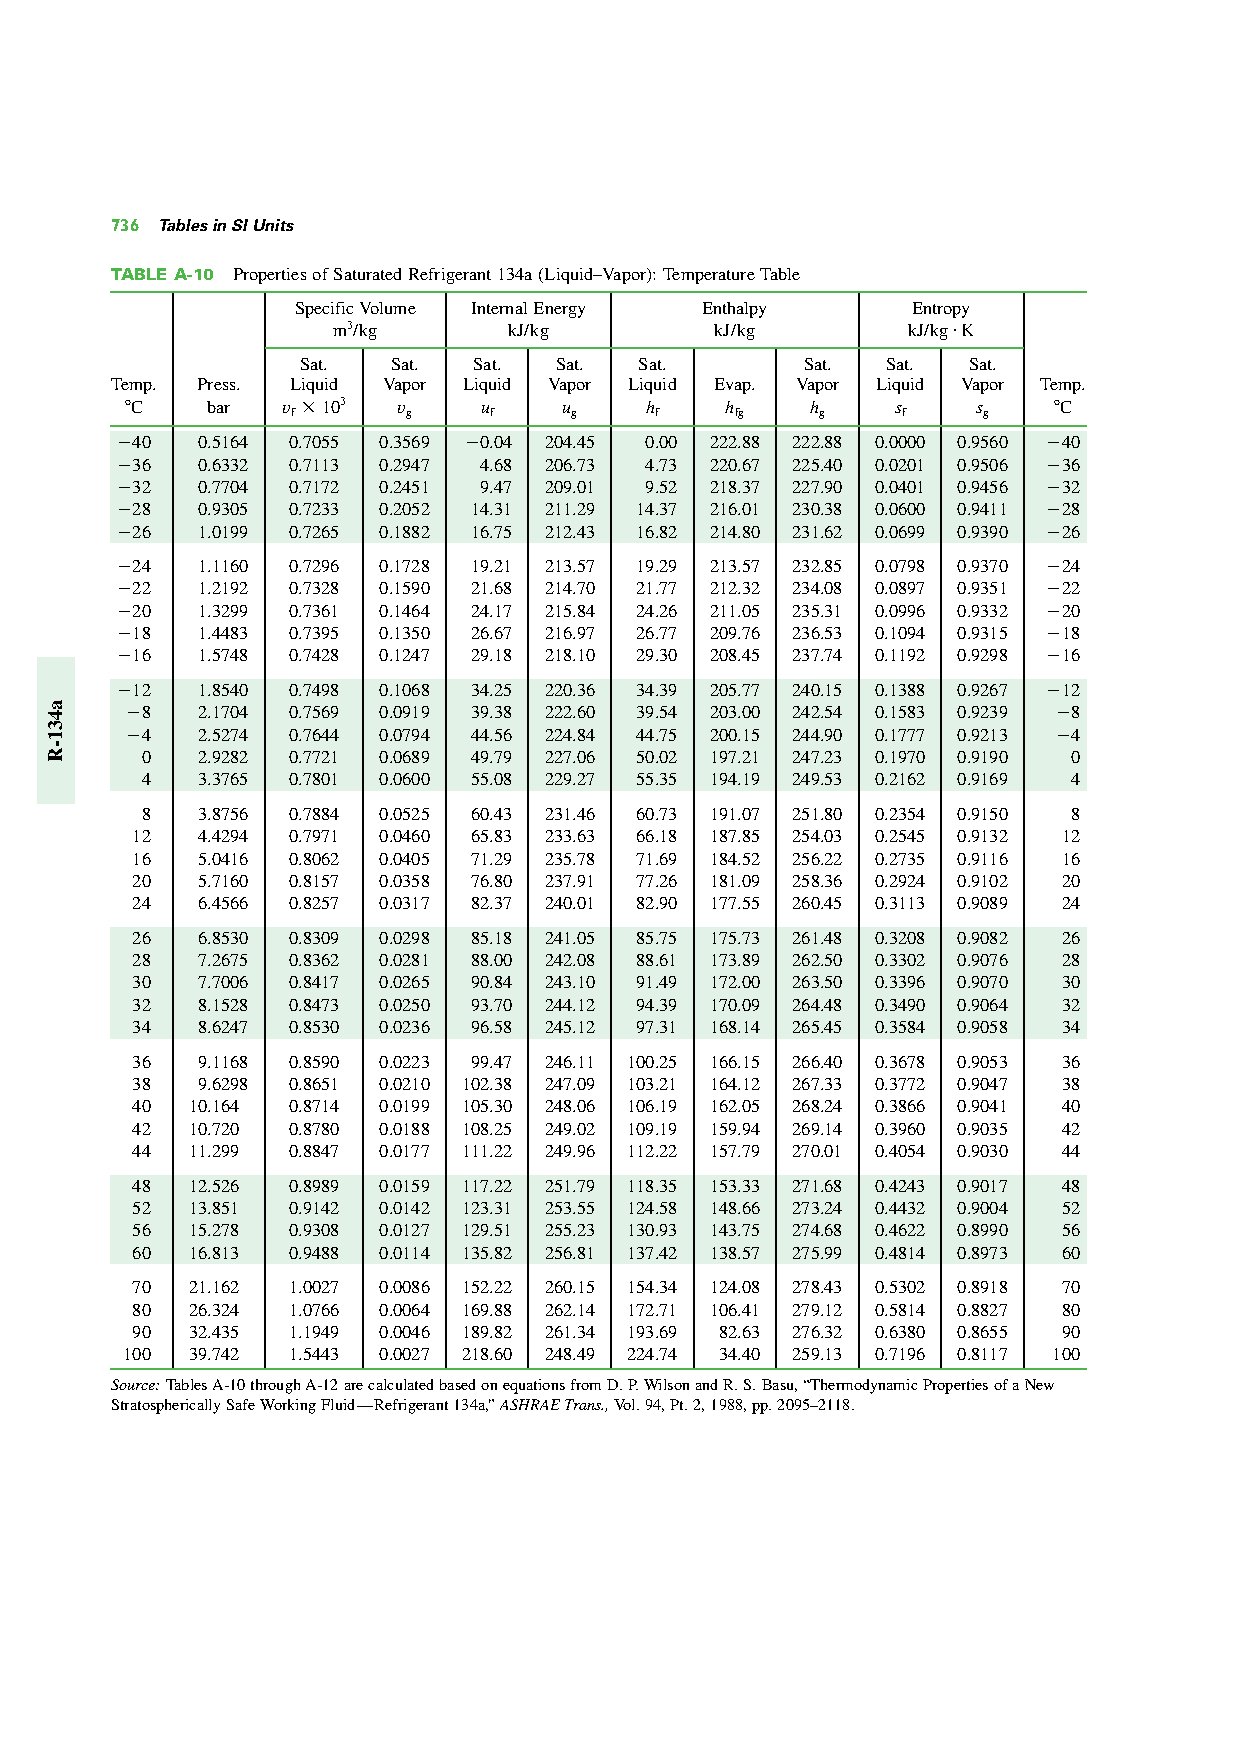
\includepdf[pages=-,fitpaper]{./Pics/Tables_R134}
}
%\end{landscape}
%\end{comment}

\end{document}
